\documentclass[12pt]{article} 
\usepackage[xetex, a4paper, left=2cm, right=2cm, top=2cm,bottom=2cm]{geometry}
\usepackage[cm-default]{fontspec}
\usepackage{xunicode}

%\tolerance=1000
%\emergencystretch=0.74cm 

\usepackage{polyglossia}
\setdefaultlanguage[spelling=modern]{russian}
\setotherlanguage{english} 
\defaultfontfeatures{Scale=MatchLowercase,Ligatures=TeX}  %% устанавливает поведение шрифтов по умолчанию  
\newfontfamily\cyrillicfont{Linux Libertine} 
\setromanfont[Mapping=tex-text]{Linux Libertine}
\setsansfont[Mapping=tex-text]{Linux Biolinum}
\setmonofont{DejaVu Sans Mono}
%\newfontfamily\cyrillicfont{Liberation Mono} 

%\usepackage{makecell}

%\usepackage{titlesec}
%\newcommand{\sectionbreak}{\clearpage}

%\renewcommand{\thesection}{\Alph{section}}
%\newcount\wd    \wd=\textwidth \multiply\wd by 8 \divide\wd by 17

\usepackage{minted}
\usemintedstyle{friendly}
\renewcommand\listingscaption{Код}
\newminted{bash}{frame=lines}
\newminted{c}{frame=leftline}

\usepackage[unicode, pdfborder={0 0 0 0}]{hyperref}

\author{Alaksiej Stankievič}
\title{Домашнее задание}

\begin{document}
\hypersetup{
pdftitle = {Задание 16},
pdfauthor = {Alaksiej Stankievič},
pdfsubject = {домашнее задание}
}% End of hypersetup

\section{Сортировки массивов}
\subsection{Оценка времени работы алгоритмов.}
Одним из значимых критериев, по которому оценивается программный продукт, является эффективность. Под эффективностью, в свою очередь, скрывается несколько параметров, среди которых нас будет интересовать скорость. Исторически сложилось оценивать скорость временем работы. Можно, конечно, напрямую указать время работы в секундах или других единицах  измерения времени, но такая величина будет очень сильно зависеть от машины, которая выполняет программу, поэтому такие оценки используют только для сравнения готовых программных продуктов с указанием конкретной тестирующей машины. Кроме того, на непосредственное время работы влияет несколько факторов: эффективность алгоритма, эффективность кодирования алгоритма, эффективность компилятора/интерпретатора и эффективность машинных команд данного процессора. Программист может существенно повлиять лишь на первые два фактора, однако увеличение эффективности кодирования алгоритма состоит в "недопускании глупостей", что достигается очень быстро. Поэтому наиболее важный 
вклад, который вносит программист, это выбор или разработка наиболее эффективного алгоритма для данной задачи.

Время работы алгоритма зависит от размера задачи (входных данных). Можно пойти двумя путями: ввести аналог скорости либо получить зависимость времени от размера входных данных. Разработчики алгоритмов выбрали второй вариант. Получать и представлять эту зависимость можно по-разному.  Например, можно посчитать количество всех действий (сложений, умножений и сравнений) в зависимости от размера, или только умножений (так как они часто медленнее сложений). Но такую зависимость получить достаточно сложно, к тому же она несёт много избыточной информации. Со временем выработался общепринятый подход: сравнивать асимптотическое поведение этих зависимостей. В матанализе вы уже встречали способы выражения асимптотического поведения, например:
\begin{equation}
f(n)\in{}O(g(n)) \Leftrightarrow{} \exists{n_{0}, c>0}, \forall{n>n_{0}}: f(n)\leq{}cg(n).
\end{equation}
Часто, хотя это менее математически строго, пишут $f(n)=O(g(n))$. В оценке алгоритмов также используются следующие асимптотики
\begin{equation}
f(n)\in{}\Theta(g(n)) \Leftrightarrow{} \exists{n_{0},c_{1},c_{2}>0}, \forall{n>n_{0}}:0\leq{}c_{1}g(n)\leq{}f(n)\leq{}c_{2}g(n),
\end{equation}
\begin{equation}
f(n)\in{}\Omega(g(n)) \Leftrightarrow{} \exists{n_{0},c>0}, \forall{n>n_{0}}:0\leq{}cg(n)\leq{}f(n).
\end{equation}

Очень важной среди них является $\Theta()$, так как она устанавливает и нижнюю, и верхнюю границу асимптотического поведения, однако часто нам нужна лишь верхняя граница, поэтому во многих статьях употребляется $O()$, что провоцирует неверное употребление $O()$ в качестве $\Theta()$.

Рассмотрим примеры оценок времени работы. Поиск максимума в произвольном массиве можно осуществить за $O(n)$, поиск произвольного элемента тоже за $O(n)$, а в уже отсортированном массиве за $O(\log{}n)$. Ясно, что поиск в отсортированном массиве происходит быстрее, но на саму сортировку нужно затратить много времени. Так уже известная нам обменная сортировка (метод пузырька) тратит $\Theta(n^{2})$. Алгоритмы сортировок не использующие особенности данных, а лишь попарные сравнения в наихудшем случае работают за $ \Omega(n\log{n}) $\footnote{См. например, Кормен Т. Алгоритмы: построение и анализ.}.

Кроме времени выполнения важным ресурсом также является память, разумеется, для хранения данных всегда нужна память $O(n)$, но для работы не которых алгоритмов нужна дополнительная память, этот факт здесь будет обозначаться $+M_{em}=\Theta(g(n)) $ после времени работы алгоритма.
\subsection{Сортировка слиянием.}
Время работы и память $ \Theta(n\log{n})+M_{em} =\Theta(n)$. Этот алгоритм построен по принципу «разделяй и властвуй». Массив делится несколько раз пополам, пока не останутся массивы из одного элемента, которые естественно отсортированы, затем отсортированные массивы сливаются  (отсюда название).

Алгоритм в псевдокоде\footnote{Псевдокод — это такое представление алгоритма, которое похоже на какой нибудь язык программирование, но в тоже время неформальное и может содержать простые словесные описания действий, которые реализуются многими командами языка. Псевдокод часто удобней чистого кода при изучении алгоритма, так как позволяет сосредоточится на сути, а не деталях. Здесь и далее будет использован либо псевдокод похожий на С/С++, либо словесное описание алгоритма. Хочу обратить внимание, что в противоположность стилю C/C++, подпрограммы я пишу с большой буквы, но в реальных программах я по прежнему советую всё начинать с маленькой буквы.}:
\begin{verbatim}
MergeSort(массив ar, начало l, конец r){
   if(l<r){
      MergeSort(ar,l,(r+l)/2);
      MergeSort(ar,(r+l)/2+1,r);
      скопировать массив ar[l,(r+l)/2] в массив br;
      скопировать массив ar[(r+l)/2+1,r] в массив cr;
      установить i, j, k на начало ar[l,r], br, cr соответсвенно;
      while(j и k в границах своих массивов){
         if(br[j]<cr[k]){
            a[i]=br[j];
            ++j;
         }else{
            a[i]=cr[k];
            ++k;
         }
         ++i;
      }
      оставшийся массив скопировать в конец ar;
   }
}
\end{verbatim}
Отметим, что данный алгоритм использует рекурсивный вызов, это довольно типичная черта алгоритмов «разделяй и властвуй».
\subsection{Пирамидальная сортировка.} Время работы $ \Theta(n\log{n})$. Это очень интересный алгоритм и в своей сути не
 сложный алгоритм, но чтобы понять, как он работает, требуется усвоить дополнительную теоретическую конструкцию.

Пирамидой или кучей\footnote{от англ. \textit{heap} — куча. Здесь следует отметить, сложившуюся терминологическую
неразбериху русских переводов: английское слово используются и для названия структуры, и для механизма распределения
памяти в системе со сборкой «мусора» (который часто используют пирамиду для её организации). Но если английское слово
равноправно несёт и смысл горы, пирамиды, и смысл мусора, то русское слово гораздо теснее связано с мусором, поэтому
структуру лучше обозначать словом более сосредоточенным на форме.} называется двоичное дерево особого вида: все уровни,
кроме, может быть, последнего заполнены и предок старше обоих потомков. Последнее свойство называется также основным
свойством пирамиды.

\begin{center}
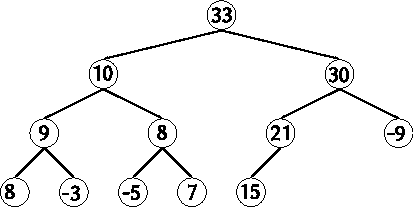
\includegraphics{fig1.pdf}

\textbf{Пример пирамиды}
\end{center}
\begin{center}

\includegraphics{fig2.pdf}

\textbf{Соответствие между пирамидой и массивом}
\end{center}

Из основного свойства пирамиды вытекает, что в корне должен находится максимальный элемент. Число элементов пирамиды
называется размером пирамиды, а число уровней высотой пирамиды. Существует однозначное соответствие между массивом и
пирамидой: корень пирамиды является первым элементом массива (нулевой индекс), а формула $ 2i+1 $ и $ 2i+2 $ задаёт
соответственно левого и правого потомка\footnote{$i$ — индекс массива как в С/С++}. Если существует почти правильная
пирамида, то есть пирамида, для которой выполняется основное свойство пирамиды для всех узлов кроме одного, то такую
пирамиду легко исправить за время $ O(\log{}n) $. Алгоритм восстановления пирамиды выглядит следующим образом:
\begin{verbatim}
Repair(A,i) {
  l=левый_потомок(i);
  r=правый_потомок(i);
  larg=i;
  if(l<размер_пирамиды(А)&&A[l]>A[larg])larg=l;
  if(r<размер_пирамиды(А)&&A[r]>A[larg])larg=r;
  if(larg!=i) {
    Обменять местами A[larg] и A[i];
    Repair(A,larg);
  }
}
\end{verbatim}
Обращаю внимание на рекурсивный вызов данной функции.

Из произвольного массива пирамида может быть построена за $ O(n) $ операций, с помощью описанного выше алгоритма
восстановления пирамиды:
\begin{verbatim}
Build(A) {
  for(i=размер_пирамиды(А)/2; i>=0; --i)
      Repair(A,i);
}
\end{verbatim}

Как уже отмечалось в построенной пирамиде первый элемент это максимальный элемент массива, следовательно он должен стоять на последнем месте. Достаточно поменять эти элементы местами, и произвести исправление пирамиды.
\begin{verbatim}
Sort(A) {
  Build(A);
  for(i=длина_массива(А)-1; i>=1; --i)
  {
    Обменять местами A[0] и A[i];
    --размер_пирамиды(А);
    Repair(A,0);
  }
}
\end{verbatim}
Обращаю внимание на уменьшение размера пирамиды.

\subsection{«Быстрая» сортировка.} Время работы алгоритма находится в пределах $ \Omega{}(n\log{}n) $ и $ O(n^{2}) $.
То есть данный алгоритм асимптотически неустойчив, в зависимости от входных данных, он может работать с любой
асимптотикой из указанных пределов. Но для случайных данных он в среднем выполняется за $ \Theta(n\log{}n) $.
Существуют несколько модификаций этого алгоритма, различие которых состоит в процедуре разбиения. Алгоритм в своей сути
реализует подход «разделяй и властвуй», также как и сортировка слиянием. Но если в сортировке слиянием всегда происходит
деления массива на две равные части, то в быстрой сортировке эти части произвольны\footnote{собственно мы получили бы
устойчивую хорошую асимптотическую оценку, если бы смогли добиться того, что  разбиение производилось бы на две равные
части}. Суть процедуры разбиения состоит в том, что бы выбрав какой либо опорный элемент произвести манипуляции над
массивом такие, что опорный элемент займёт тоже место что и отсортированном массиве: все элементы левее будут меньше,
все элементы праве будут больше\footnote{в случае сортировки по возрастанию}. В дальнейшем мы производим рекурсивное
выполнение данного алгоритма к оставшимся частям. Как и раньше массив из одного элемента отсортирован.
\begin{minted}{cpp}
Sort(A,l,r) {
  if(l<r) {
    m=Partition(A,l,r);
    Sort(A,l,m-1);
    Sort(A,m+1,r);
  }
}
\end{minted}

Вот один из возможных вариантов процедуры разбиения, когда в качестве опорного элемента выбран последний элемент
массива\footnote{без рандомизаци это очень плохой выбор опорного элемента, так как уже отсортированный массив будет
обрабатываться по худшему случаю}:
\begin{verbatim}
Partition(A,l,r){
  i=l;
  while(A[i]<A[r])++i;
  for(j=i;j<r;++j)
    if(A[j]<A[r]){
      Обменять местами A[j] и A[i];
      ++i;
    }
  Обменять местами A[i] и A[r];
  return i;
}
\end{verbatim}
Чтобы получить другие модификации разбиения\footnote{материал для самостоятельного изучения в сети Интернет} можно
найти по какому либо принципу опорный элемент, поставит его на последнее место, а затем применить уже описанную
процедуру разбиения. Оформление в данном случае процедуры разбиения в виде отдельной функции является неоптимальным, и
лучше данную процедуру вставить непосредственно в код быстрой сортировки. Исходный массив сортируется вызовом сортировки
от граничных индексов исходного массива.


\section{Задание}

Реализовать все указанные ниже сортировки, в заголовочном файле должно быть прописаны прототипы функций сортировки,
которые получаю массив и размер. Проведите измерение времени выполнения различных сортировок. Программа должна быть
аккуратно организована и оформлена.

\begin{enumerate}
 \item Сортировка выбором (selection).
 \item Сортировка обменом (пузырьковая) (buble).
 \item Сортировка вставками (insertion).
 \item Сортировка слиянием (merge).
 \item <<Быструю>> сортировку (quick).
 \item Пирамидальную (heap).
\end{enumerate}

Для получения бонуса можно реализовать:

\begin{enumerate}
 \item Introsort
 \item Сортировку Тима (timsort).
\end{enumerate}

\section{Задание}

Реализовать одно из двух на выбор (или оба для получения бонуса).

\begin{enumerate}
 \item Трёхмерные крестики нолики, в кубе $4\times 4 \times 4$. Побеждает игрок выстроивший линию из 4. Куб рисуется по
этажам.
 \item Плоские крестики нолики на большом поле (минимум $20 \times 20$). Побеждает игрок выстроивший линию из 5.
\end{enumerate}

\subsection{Совет}
Мне видится удобным для упрощения проверок на выигрыш реализовать функцию проверки одной линии следующей сигнатуры:
\begin{listing}[H]
\begin{center}
\begin{ccode}
int checkLine(int field[][4][4], int length, int i, int j, int k,
                int vi, int vj, int vk);
\end{ccode}
\end{center}
\caption{Проверка одной линии}
\label{lst:checkline}
\end{listing}
Функция возвращает 0, если на линии нет победителя, 1 если линия заполнена ноликами, 2 если крестиками. Параметр field
это игровое поле (в коде \ref{lst:checkline}, рассмотрен случай трёхмерных крестиков ноликов, в плоских всё похоже).
Параметр length это длина линии\footnote{В принципе её можно зашить в код функции, но так получается более
масштабируемое (особенно для плоского случая) решение.}. Параметры i, j, k это индексы начальной ячейки линии. А
параметры vi, vj, vk определяют куда линия направлена\footnote{С математической точки зрения это не что иное, как
координаты направляющего вектора, отсюда и название параметров}, они могут принимать только три значения -1, 0 и 1.
Например, рассмотрим случай когда $(i, j, k) = (0, 0, 0)$ и $(vi, vj, vk) = (1, 1, 0)$, тогда первая ячейка линии $(0,
0, 0)$, вторая ячейка получается из первой прибавлением соответствующих компонент $v$, а именно в нашем случае $(1, 1,
0)$, третья --- прибавлением компонент $v$, что даёт $(2, 2, 0)$ и четвёртая в итоге $(3, 3, 0)$, то есть мы получили
диагональную линию на этаже с индексом 0. Если $(vi, vj, vk) = (1, 0, 0)$, то получится вертикальная линия на этаже с
индексом 0, а если $(vi, vj, vk) = (1, 1, 1)$, то получится диагональ через весь куб.



\end{document}
